\chapter{Analiza wyników badań}
\label{results}
\section{Dane testowe}
\par{
  Przygotowanie zestawu danych testowych jasno odzwierciedlającego ograniczenie złożoności obliczeniowej rozwiązania problemu pokrycia wierzchołkowego do wielomianowej przez zastosowanie technik redukcji dziedziny do jądra problemu nie jest łatwe.
  Opisywane techniki bardzo silnie zależą od charakterystycznych cech struktury grafu, które ciężko jest opisać w prosty sposób parametrami generacji losowej.
  Dlatego też aby przygotować zestaw losowych grafów testowych przyjęto metodę generacji opartą o rozkład losowy stopni wierzchołków grafu w połączeniu z funkcją określającą współczynnik selektywności.
  Stopień każdego wierzchołka w generowanym grafie wybierany jest losowo z przedziału $\left<1, k\right>$ zgodnie z rozkładem $P(k) \propto \frac{1}{k}$.
  Uzyskanie zbioru grafów losowych o różnych parametrach owocowało bardzo niespójnymi wynikami czasów ich przetwarzania z pomocą opisywanych w niniejszej pracy technik, co spowodowane jest tym, że istnienie struktur redukowalnych w grafie nie jest uzależnione wprost od liczebności wierzchołków czy też krawędzi.
  Po ``wypróbowaniu'' kilku postaci funkcji określającej współczynnik selektywności udało się utworzyć zbiór zapewniający na zbliżone do oczekiwanych pod względem przyrostu czasu przetwarzania wyniki --- przyjęta została postać $P(i, k) \propto \frac{1}{1+|i-k|}$, gdzie $i$ stanowi stopień rozpatrywanego wierzchołka.
  Następnie, w celu uściślenia monotoniczności wyników, metodą prób i błędów dobrano wartość parametru $k=5$.
  Dla tak wybranych parametrów wygenerowano przedstawiony w~Tabeli~\ref{tab_testdata} zbiór grafów $G=(V, E)$, mających pokrycia wierzchołkowe $C$.\\
  \begin{table}
    \begin{center}
    \begin{tabular}{| c | c | c | c |}
      \hline
      l.p. & $|V|$ & $|E|$ & $|C|$ \\ \hline
      1 & 100 & 115 & 47 \\
      2 & 200 & 246 & 96 \\
      3 & 300 & 367 & 152 \\
      4 & 400 & 508 & 199 \\
      5 & 500 & 589 & 241 \\
      6 & 600 & 744 & 290 \\
      7 & 700 & 860 & 348 \\
      8 & 800 & 964 & 396 \\
      9 & 900 & 1113 &  445 \\
      10 & 1000 &  1218 &  501 \\ \hline
    \end{tabular} 
    \begin{tabular}{| c | c | c | c |}
      \hline
      l.p. & $|V|$ & $|E|$ & $|C|$ \\ \hline
      11 & 1100 & 1360 &  543 \\
      12 & 1200 & 1446 &  590 \\
      13 & 1300 & 1571 &  651 \\
      14 & 1400 & 1717 &  693 \\
      15 & 1500 & 1758 &  739 \\
      16 & 1600 & 2010 &  804 \\
      17 & 1700 & 2079 & 1018 \\
      18 & 1800 & 2219 & 1095 \\
      19 & 1900 & 2326 & 1119 \\
      20 & 2000 & 2463 & 1163 \\ \hline
    \end{tabular}
    \end{center}
    \caption{Wartości opisujące grafy stanowiące zbiór danych testowych.}
    \label{tab_testdata}
  \end{table}
}
\section{Porównanie i analiza wydajności opisanych algorytmów}
\par{
  W celu zbadania efektywności zaimplementowanych algorytmów wykonano serię testów, podczas których mierzono czas wykonywania nsatępujących operacji.
  \begin{itemize}
    \item Wyznaczenie pokrycia wierzchołkowego metodą naiwną dla zestawu grafów o pomniejszonych rozmiarach.
    \item Wyznaczenie pokrycia wierzchołkowego algorytmem własnym, opisanym Pseudokodem~\ref{alg_VC2}.
    \item Wyznaczenie pokrycia wierzchołkowego algorytmem własnym po redukcji koron.
    \item Wyznaczenie pokrycia wierzchołkowego algorytmem własnym po rozwiązania przeformułowania problemu jako egzemplarza problemu przepływu w sieci.
    \item Wyznaczenie pokrycia wierzchołkowego algorytmem własnym po wykonaniu operacji przetwarzania wstępnego i redukcji koron.
    \item Wyznaczenie pokrycia wierzchołkowego algorytmem własnym po wykonaniu operacji przetwarzania wstępnego i rozwiązania przeformułowania problemu jako egzemplarza problemu przepływu w sieci.
    \item Redukcja dziedziny do jądra problemu poprzez usunięcie koron.
    \item Redukcja dziedziny do jądra problemu poprzez rozwiązanie przeformułowania problemu jako egzemplarza problemu przepływu w sieci.
  \end{itemize}
}
\subsection{Wyznaczanie pokrycia wierzchołkowego}
\par{
  Zgodnie z oczekiwaniami, wyznaczenie pokrycia wierzchołkowego metodą siłową, opisaną Pseudokodem~\ref{alg_VC1} wymagało wykładniczej ilości czasu.
  Powoduje to, że analiza grafów o rozmiarach przedstawionych w Tabeli~\ref{tab_testdata} trwa bardzo długo, a wyniki pomiarów związanych z metodą siłową zaciemniają obraz wyników pozostałych testów.
  W związku z tym pomiar czasu działania metody siłowej zrealizowany miał zostać dla osobnego zestawu siedmiu grafów o rozmiarach od dziesięciu do trzydziestu wierzchołków wygenerowanych opisaną metodą.
  Niestety, struktura jednego z wygenerowanych grafów okazała się być niekorzystna dla rozgałęzień algorytmu siłowego --- wyniki pomiarów czasu działania siłowej metody wyznaczania pokrycia wierzchołkowego zawiera Tabela~\ref{tab_vc_naive}.
  \begin{table}
    \begin{center}
      \begin{tabular}{| c | c | c | c |}
        \hline
        l.p. & $|V|$ & $|E|$ & czas \\ \hline
        1 & 10 & 8 & 323.884$\mu$s \\
        2 & 15 & 20 & 9.52204ms \\
        3 & 20 & 20 & 30.605758ms \\
        4 & 25 & 33 & 614.454963ms \\
        5 & 30 & 36 & 28.922161504s \\
        6 & 35 & 35 & 1m27.328533967s \\
        7 & 40 & 69 & \textit{wyłączono po 2 godzinach} \\ \hline
      \end{tabular} 
    \end{center}
    \caption{Czas wyznaczania pokrycia wierzchołkowego metodą siłową.}
    \label{tab_vc_naive}
  \end{table}
  \begin{figure}
    \caption{Czas działania siłowej metody wyznaczania pokrycia wierzchołkowego grafu.}
    \label{fig_results_naive}
    \centering
      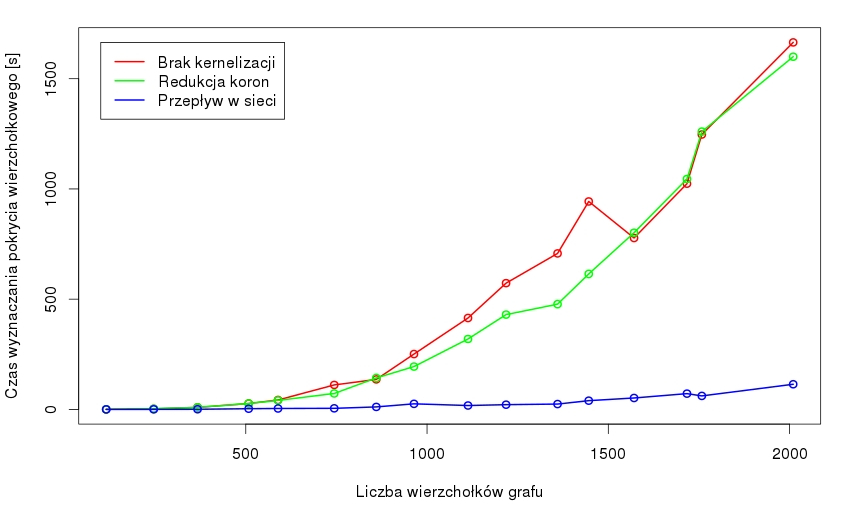
\includegraphics[width=\textwidth]{results-naive}
  \end{figure}
}
\subsubsection{\textbf{Czas wyznaczania pokrycia wierzchołkowego bez przetwarzania wstępnego}}\label{time_vc}
\par{
  Porównanie czasów wyznaczania pokrycia wierzchołkowego bez uprzedniego zastosowania technik przetwarzania wstępnego przedstawia Rysunek~\ref{fig_results_vc}.
  \begin{figure}
    \caption{Czas wyznaczania pokrycia wierzchołkowego bez przetwarzania wstępnego.}
    \label{fig_results_vc}
    \centering
      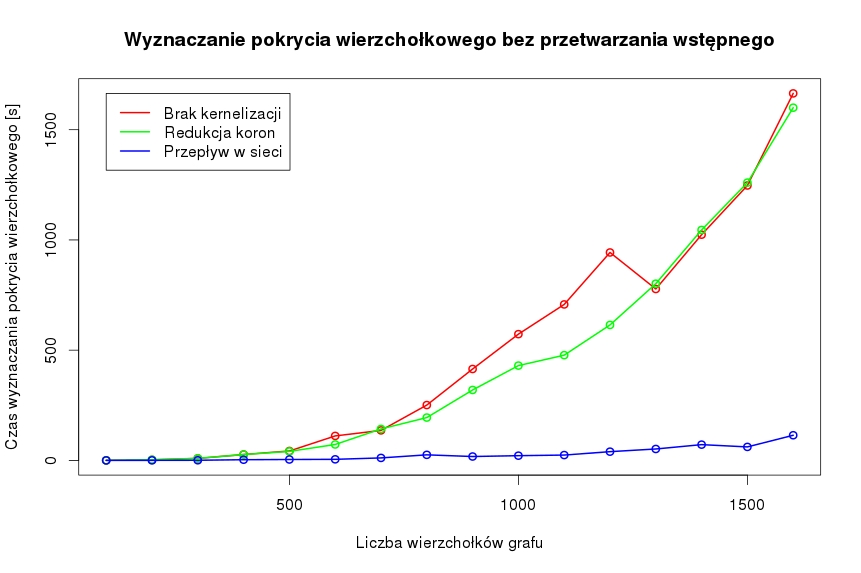
\includegraphics[width=\textwidth]{results-vc}
  \end{figure}
  Wyraźnie widoczny jest pozytywny wpływ zastosowania redukcji dziedziny do jądra problemu przez rozwiązanie przeformułowania problemu do egzemplarza problemu przeływu w sieci.
  Jako prawdopodobne uzasadnienie tego, że redukcja koron nie oferuje tak dużego przyspieszenia jak technika oparta na przepływie w sieci uznano dwa powody.
  \begin{itemize}
    \item Grafy stanowiące dane testowe są ubogie w korony.
    Wynika to z postaci funkcji określającej współczynnik selektywności wierzchołków --- struktury koron wymagają bardzo specyficznych relacji zachodzących pomiędzy zbiorami wierzchołków, mianowicie istnienia zbiorów niezależnych o połączonym sąsiedztwie.
    W ramach procesu przygotowywania danych testowych udało się uzyskać grafy, dla których redukcja dziedziny uzyskana przez usunięcie koron była znacznie większa, jednak grafy te nie pozwalały na uzyskanie wyników dających przedstawić się w postaci funkcji zachowującej choćby pozory monotoniczności.
    \item Zaimplementowana technika wyznaczania koron w grafie oparta jest na zbyt restrykcyjnym uściśleniu NT--redukcji do serii operacji działających bezpośrednio na konkretnych egzemplarzach skojarzeń.
    Najprawdopodobniej stanowi to również powód opisanych w podrozdziale~\ref{sss_problems_ckx} problemów napotkanych przy implementacji algorytmu Chen, Kanj, Xia.
    Pozostałe zaimplementowane egzemplarze NT--redukcji wyznaczają podzbiory różniące się od tych uzyskiwanych przez redukcję proponowaną w pracy~\cite{KernelizationAlgorithms04}.
    Dalsze pole do badań może stanowić weryfikacja czy bardziej ogólne postacie NT--redukcji --- wykonywane za pomocą algorytmów programowania liniowego --- zapewnią lepsze rezultaty dla grafów o strukturze zbliżonej do tych, które wykorzystano jako dane testowe.
  \end{itemize}

  Ze względu na niedoskonałości implementacji opisywanych w niniejszej pracy nie udało się wykonać pomiarów czasu wyznaczania pokrycia wierzchołkowego bez przetwarzania wstępnego dla grafów zawierających więcej niż 1600 wierzchołków.
  Pomimo nieco gorszych od oczekiwanych rezultatów należy zauważyć, że każda z przedstawionych charakterystyk jest o wiele rzędów wielkości lepsza niż charakterystyka uzyskana z pomiarów czasu działania metody siłowej.
}
\subsubsection{\textbf{Czas wyznaczania pokrycia wierzchołkowego po przetwarzaniu wstępnym}}
\par{
  Porównanie czasów wyznaczania pokrycia wierzchołkowego po uprzednim zastosowaniu technik przetwarzania wstępnego przedstawia Rysunek~\ref{fig_results_vc_p}.
  \begin{figure}
    \caption{Czas wyznaczania pokrycia wierzchołkowego po przetwarzaniu wstępnym.}
    \label{fig_results_vc_p}
    \centering
      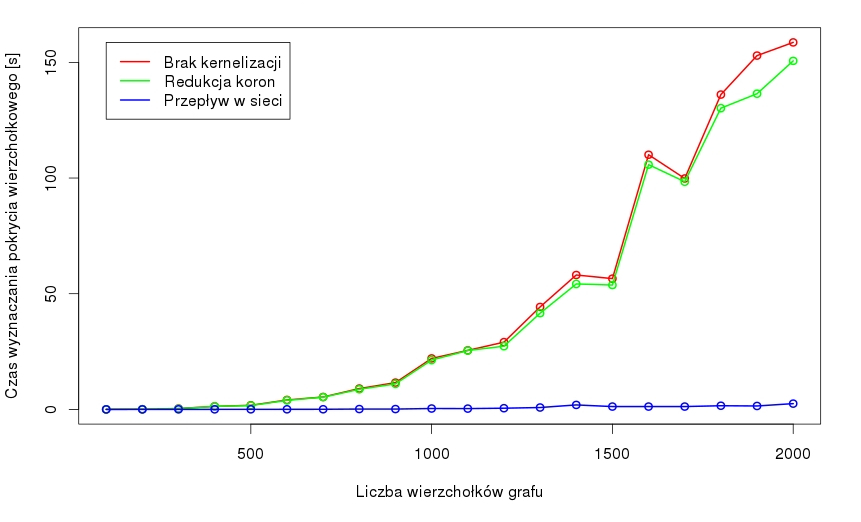
\includegraphics[width=\textwidth]{results-vc-p}
  \end{figure}
  Zastosowanie prostych technik przetwarzania wstępnego opisanych w podrozdziale~\ref{Section_preprocessing} pozwala na dodatkowe skrócenie czasu wyznaczania pokrycia wierzchołkowego w grafach testowych o około dwa rzędy wielkości.
}
\par{
  Ponieważ różnica w czasie wyznaczania pokrycia wierzchołkowego z zastosowaniem techniki opartej o przepływ w sieci pomiędzy wariantem bez przetwarzania wstępnego a wariantem z zastosowaniem przetwarzania wstępnego jest słabo widoczna, Rysunek~\ref{fig_nf_comp} zestawia charakterystyki czasowe tych przypadków.
  \begin{figure}
    \caption{Wpływ przetwarzania wstępnego na czas wyznaczania pokrycia wierzchołkowego w oparciu o przepływ w sieci.}
    \label{fig_nf_comp}
    \centering
      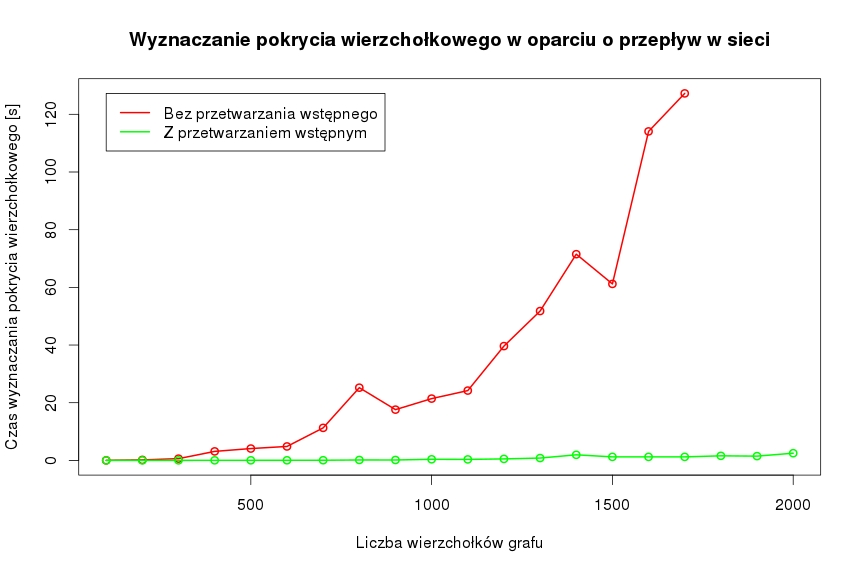
\includegraphics[width=\textwidth]{nf-comp}
  \end{figure}
}
\subsection{Algorytmy przetwarzania wstępnego i redukcji dziedziny do jądra problemu}
\par{
  Redukcja dziedziny do jądra problemu w praktyce może mieć sens jedynie wtedy, gdy czas potrzebny wykonanie operacji zawężających przestrzeń poszukiwań pokrycia wierzchołkowego jest wielomianowy.
  W celu weryfikacji szybkości działania implementacji opisywanych technik redukcji dziedziny oraz przetwarzania wstępnego zmierzono czas potrzebny na wykonanie tych operacji dla zbioru grafów testowych. 
}
\subsubsection{\textbf{Algorytmy redukcji dziedziny do jądra problemu}}
\par{
  Porównanie czasów wyznaczania pokrycia wierzchołkowego bez uprzedniego zastosowania technik przetwarzania wstępnego przedstawia Rysunek~\ref{fig_results_k}.
  \begin{figure}
    \caption{Czas redukcji dziedziny bez przetwarzania wstępnego.}
    \label{fig_results_k}
    \centering
      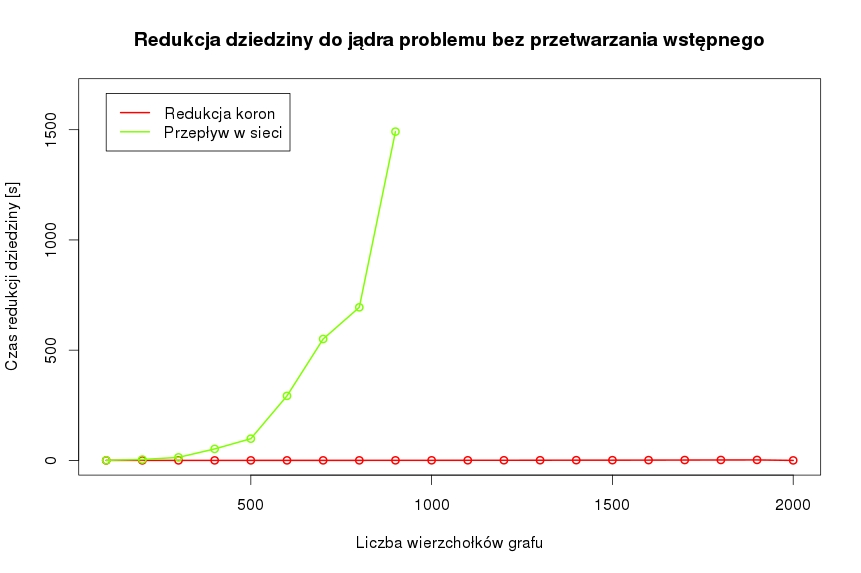
\includegraphics[width=\textwidth]{results-k}
  \end{figure}
  Powodem bardzo niekorzystnej złożoności czasowej działania algorytmu redukcji dziedziny przez rozwiązanie przeformułowania problemu do egzemplarza problemu przepływu w sieci są błędy popełnione przy implementacji koncepcji opisanej w pracy~\cite{KernelizationAlgorithms04}.
  Szczegóły tych błędów oraz proponowane usprawnienia opisane są w podrozdziale~\ref{s_improvements}.
  Ponieważ charakterystyka wyników pomiarów czasu działania tego algorytmu jest zdeformowana i nie ukazuje prawdziwej jego szybkości, a także ze względu na bardzo długi czas oczekiwania, ograniczono dziedzinę przetwarzanych przez niego grafów do zawierających najmniejszą liczbę wierzchołków.
  W związku z zaciemnieniem na wykresie wartości wyników pomiarów czasu działania algorytmu redukcji koron, Rysunek~\ref{fig_results_k_crown} przedstawia wyłącznie tę charakterystykę.
  \begin{figure}
    \caption{Czas redukcji dziedziny przez wyznaczenie i usunięcie koron bez przetwarzania wstępnego.}
    \label{fig_results_k_crown}
    \centering
      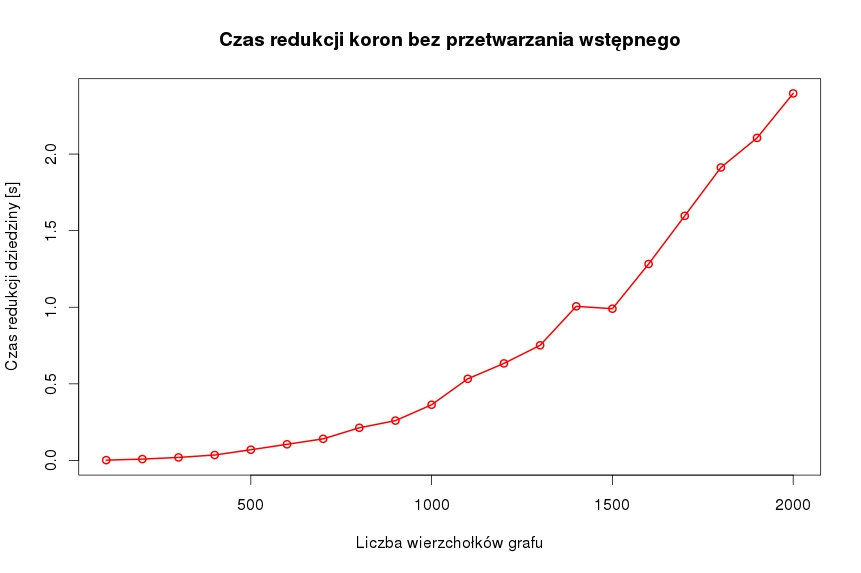
\includegraphics[width=\textwidth]{results-k-crown}
  \end{figure}
}
\par{
  Na Rysunku~\ref{fig_results_k_crown} można zauważyć gwałtowny spadek czasu działania algorytmu redukcji koron dla grafu o dwóch tysiącach wierzchołków.
  Jest on spowodowany napotkaniem przez algorytm sytuacji świadczącej o tym, że w grafie nie może istnieć korona --- prowadzi to do natychmiastowego zakończenia jego działania.
  Biorąc pod uwagę to, że zbiór grafów testowych jest efektem wielu prób przygotowania odpowiedniego zestawu danych przy doborze różnych parametrów generacji grafów, ten przypadek uświadamia jak bardzo wrażliwy na strukturę grafu jest algorytm redukcji koron.
}
\par{
  Rysunek~\ref{fig_results_k_crown_p} przedstawia wpływ uprzedniego zastosowania algorytmów przetwarzania wstępnego na czas działania algorytmu redukcji koron.
  \begin{figure}
    \caption{Czas redukcji dziedziny bez przetwarzania wstępnego.}
    \label{fig_results_k_crown_p}
    \centering
      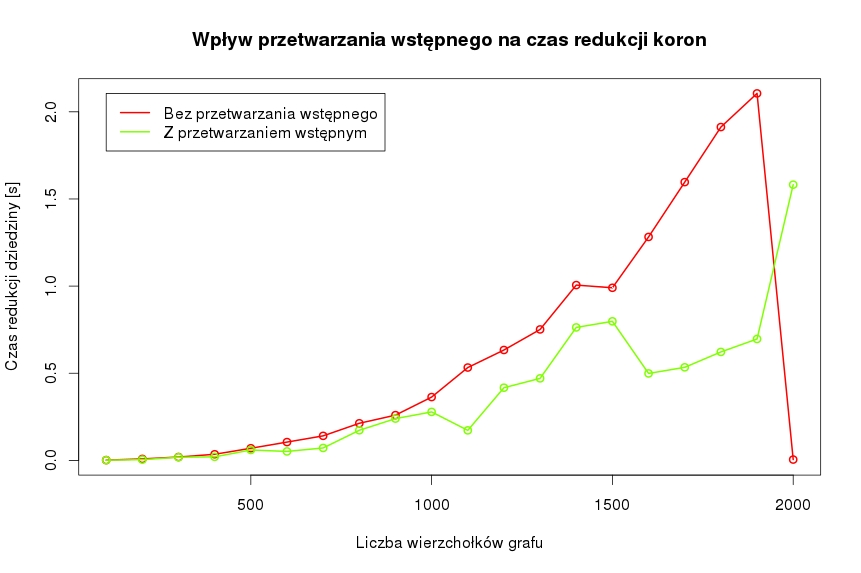
\includegraphics[width=\textwidth]{results-k-crown-p}
  \end{figure}
  Oprócz poprawy czasu działania procedury redukcji koron widać tutaj pewną zmianę w kontekście operacji na największym grafie.
  Ponieważ algorytm przetwarzania wstępnego zmienia strukturę grafu wejściowego, może prowadzić on do pojawienia się w dziedzinie struktur nie istniejących w nim wcześniej.
  Na podstawie Rysunku~\ref{fig_results_k_crown_p} można domniemać, że zwinięcie pewnego połączonego sąsiedztwa wierzchołka $v$ stopnia $d(v)=2$ w grafie wejściowym lub usunięcie pewnego wierzchołka $u$ spełniającego kryteria opisane w podrozdziale~\ref{Section_preprocessing} spowodowało pojawienie się w grafie zbiorów wierzchołków $I, H$ spełniających własności pozwalające włączyć je do korony.
  W tym wypadku przetwarzanie wstępne otwarło drogę do dodatkowej redukcji dziedziny w dalszych etapach.\footnote{Nawiązując do opisanych w podrozdziale~\ref{time_vc} problemów należy również brać pod uwagę to, że bardziej ogólna implementacja procedury redukcji korony może być w stanie wykryć rzeczone struktury nawet bez przetwarzania wstępnego dzięki algorytmowi programowania liniowego.}
}
\par{
  Rysunek~\ref{fig_results_p} przedstawia charakterystykę czasu przetwarzania wstępnego w zależności od liczby wierzchołków grafu.
  \begin{figure}
    \caption{Czas przetwarzania wstępnego.}
    \label{fig_results_p}
    \centering
      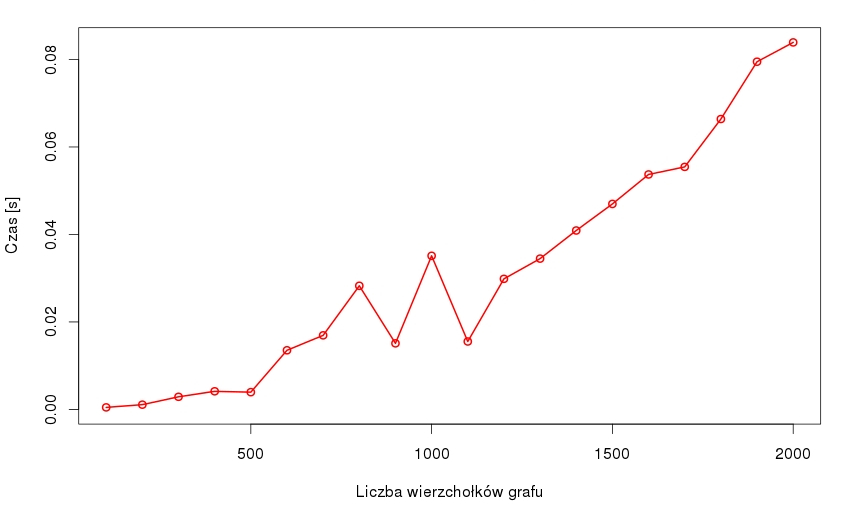
\includegraphics[width=\textwidth]{results-p}
  \end{figure}
}
\section{Wnioski}
